\chapter{Methods and materials.}

For this work, many diferent tools were used, which will be cathegorized in hardware, software and mathematical tools. \\

In terms of hardware, the author was granted access to the \textit{FQM-378} clusters in the Universidad de Córdoba. Access to these clusters was crucial for the calculations done throughout the work, reducing the time needed for each calculation in several orders of magnitude. Besides the clusters, the author also needed his own personal computer, mainly to remotely access the clusters and also for other types of calculations that could not have been done from the clusters. These calculations include among other things, plotting of figures.  \\

The main mathematical tool for this work was the Fourier Transform. The Fourier Transform is a consequence of Fourier's Theorem. This theorem states that for every `nice'\footnote{The conditions for which this theorem does not apply are beyond the scope of this work, and so the `niceness' of a function need not be defined} periodic function $f(x)$ of period $L$ one can find a unique linear combination of sine and cosine functions such that 
\begin{align}
	f(x) = C + \sum_\text{n odd} a_n \sin\left( \frac{nx}{L} \right) + \sum_{\text{n even}}^{} b_n \cos \left( \frac{nx}{L} \right) 
\end{align}
With $C $, $a_n$, $b_n$ given by 
\begin{align}
	\begin{cases}
		C &= \frac{1}{L} \int_{L}^{0} f(x) dx\\
		a_n &= \frac{1}{L} \int_{L}^{} f(x) \sin\left(  2\pi \frac{nx}{L} \right) dx,~\text{n odd}\\
		b_n &= \frac{1}{L} \int_{L}^{} f(x) \cos\left(  2\pi \frac{nx}{L} \right) dx,~\text{n even}\\
	\end{cases}
\end{align}

This was the original Fourier's result. However this theorem can be expanded to the complex realm as 
\begin{align}
	f(x) = \sum_{n=0}^{\infty} c_n e^{i 2\pi \frac{nx}{L}}, \text{with } c_n = \frac{1}{L}\int_{L}^{} f(x) e^{-i 2\pi \frac{nx}{L}}dx 
\end{align}
For each mode $n$ one can define a new variable $k=2\pi n /L$, leading to the actual definition of the Fourier Transform 
\begin{align}
	\tilde{f}(k) = \frac{1}{2\pi}\int_{L}^{}  f(x) e^{-i k x} dx
\end{align}
In this work, the power spectrum $P(k)$ is considered, which is the Fourier Transform of the correlation function $\xi(r)$.  Recalling the definition of the $\xi(r)$ function, the frequency of the distance at which two any two galaxies are found, one can notice that  $\xi(r)$ must be a discrete function. We thus define the Discrete Fourier Transform (DFT) over a discrete set of N data points $\{\left( x_i, \xi(x_i) \right) \}_{i=1}^{N} $
\begin{align}
	P(k_j) = \frac{1}{2\pi}\sum_{i=1}^{N} e^{-i k_j x_{i}} \xi(x_i)
	\label{eq:DFT}
\end{align}
Though one must think that the repeating function hypothesis is being broken, since of course the universe is not made of repeating blocks of the galaxies that surround us. That the universe is infinitely big and repeating is an assumption that needs to be done in order to calculate this Fourier Transform. In other words, these calculations asume periodic boundary conditions.


Another thing to be noted is the fast growing complexity of the algorithm described by \eqref{eq:DFT}, which grows as $N^2$, with $N$ the number of points used for the calculation. 
To solve this one would yous the Fast Fourier Transform (FFT), instead of the DFT. This algorithm is based in the decomposition of the space considered with $N=N_1N_2$ data points, into two smaller spaces with $N_1$ and $N_2$ data points. It then factorizes each problem into smaller problems, and finally only having to compute very simple DFT's. Thus reducing the complexity of the algorithm from $N^2$ to $N\log N$. 

Having vaguely introduced the $P(k)$, it can be now properly defined. Let  $\rho(\textbf{x})$ determine the density of galaxies at a given point. As the interest lays in the fluctuations around the density, it is only natural to be interested in the overdensity $\delta(\textbf{x})$ at some position $\textbf{x}$
\begin{align}
	\delta(\textbf{x}) = \frac{\rho\left( \textbf{x} \right) - \overline{\rho}}{\overline{\rho}}
\end{align}
From this magnitude one calculates the aforementioned correlation function $\xi(\textbf{r})$\footnote{Note only the dependency on $r = \|\textbf{r}\|$ remains, since the universe is (assumed to be) homogenous and isotropic} as 
\begin{align}
	\xi(\textbf{r}) = \left<\delta(\textbf{x}) \delta(\textbf{x}') \right> = \frac{1}{V}\int_{V}^{}  d^3 \textbf{x} \delta(\textbf{x}) \delta\left(\textbf{x} - \textbf{r}  \right) 
\end{align} with $\textbf{r} = \textbf{x} - \textbf{x}'$
And the power spectrum is then defined as its Fourier Transform  (En 1, 2, ó 3 dimensiones?)

However, just by observing one cannot calculate the distance at which galaxies are found. What can be used as a measure of the radial distance is the redshift $z$. To do this calculation one then needs three coordinates for each galaxy (as would be expected from a three dimensional universe). These coordinates will be 2 angular coordinates (the declination $\delta$ and right ascension $\alpha$) and a radial coordinate $r$ which must be calculated from $z$. For this it is needed to assume a cosmology.

In terms of software, the main tools for this work were Cosmic Linear Anisotropy Solving System (CLASS)~\cite{class}, Montepython~\cite{montepython}, Rapid foUrier STatIstics COde (RUSTICO)~\cite{rustico} and Bao and Rsd Algorithm for Spectroscopic Surveys (BRASS)~\cite{brass}. \\

The CLASS library was used for the generation of theoretical BAO power spectrums $P(k)$, which will be later explained for different $\Omega_k$. These power spectrums are calculated from a magnitude named the overdensity. 
From these power spectrums, one needs to calculate the $P_\text{smooth}(k)$, $O_{\text{lin}}(k)$ which is done with Montepython. These curves can be understood like the main components of the spectrum $P(k)$. $O_{\text{lin}}(k)$ are the pure Baryon Acoustic Oscillations, and $P_{\text{smooth}}(k)$ is the curve that, when modulated by the $O_{\text{lin}}(k)$ results in the original power spectrum $P(k)$. More precisely,
\begin{align}
	P(k) = P_{\text{smooth}}(k) O_{\text{lin}}(k)
\end{align}

\begin{figure}[t]
	\centering
	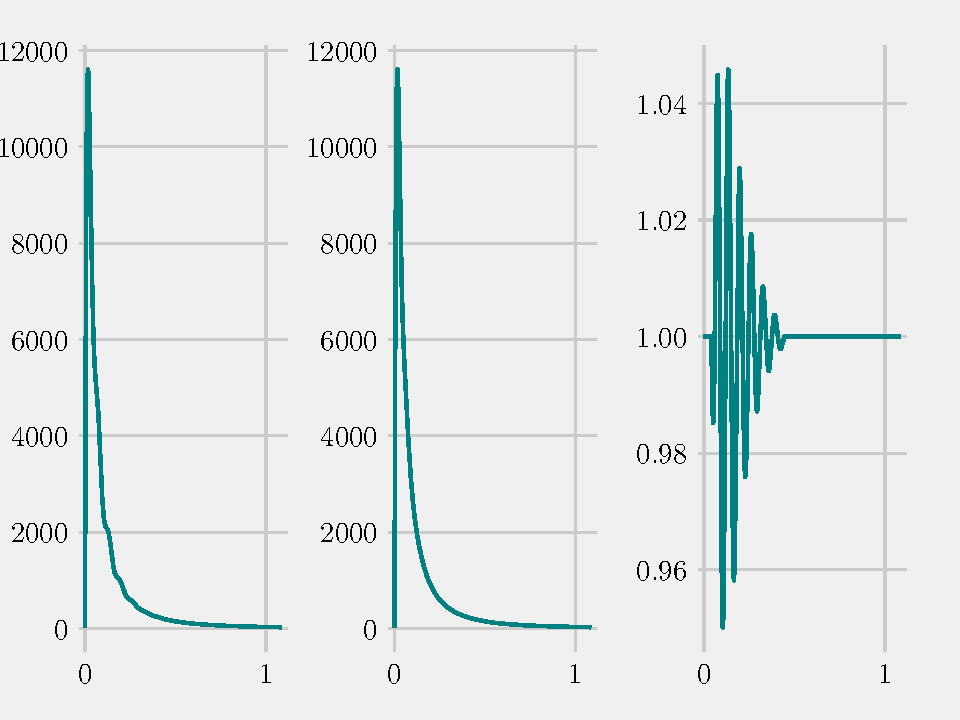
\includegraphics[width=0.8\textwidth]{../figs/PkOlPsm.pdf}
	\caption{Graphic representation of the $P(k)$, $P_{smooth}(k)$ and $O_{lin}(k)$}
	\label{fig:PkOlPsm}
\end{figure}

The RUSTICO library was used to calculate the power spectra of the galaxies measured by the LRG eBOSS measurements, again as a function of $\Omega_k$. For this, the software takes as an input the LRG eBOSS sample (citar LRG?) 
Note: Hablar de la sobre densidad (over density)P(k) es la tf de fourier de la delta. La varianza del campo es la media de la sobre densidad al cuadrado. El espectro de potencias es la varianza (como fluctua) el campo de densidad. Medido en el espacio de fourier. Hablamos de  frecuencias espaciales en vez de hablar de longitudes.

Note: Cuando hablemos de RUSTICO convertimos z->d (ley de Hubble). Con cierta cosmología podemos convertir z en r. Usamos rustico para convertir una cantidad observada (z) en r de esfrericas. Teniendo r y teniendo el angulo de cada galaxia (declinacion recta y ascension) (mirar ben) 

Note: hacemos la fft en ese cubo y calcula el campo de densidad de esos puntitos. Lo que hace es interpolar haciendo un mapa de calor tridimensional. A eso le hace la FFT y ya tenemos algo que comparar con nuestra teoría.

Note: Lo que comparamos con nuestra teoría es el segundo moemtno de la distribución. Para ello tenemos que suponer una cosmología fiducial. 

Note: Nos interesa Ok para el z->d

Note: $https://en.wikipedia.org/wiki/Matter_power_spectrum$

Note: Cuando una función es gaussiana solamente tiene definiad los dos primeros momentos, el resto son 0. Aquí la media es 0, por lo que la única que es no nula es la desviacion tipica (el 2o momento). Los densidades se crearon como campos de densidad gausianos $\implies$ solo hay media y desviación típica. La variancia de la media la llamamos xi en espacio de config y p(k) en espacio de momentos. 
